\chapter{Principal Component Analysis}


\section{Introduction}
\begin{itemize}
    \item Dimensionality Reduction

    \begin{figure}[!htbp]
        \begin{minipage}[t]{0.45\textwidth}
            \centering
            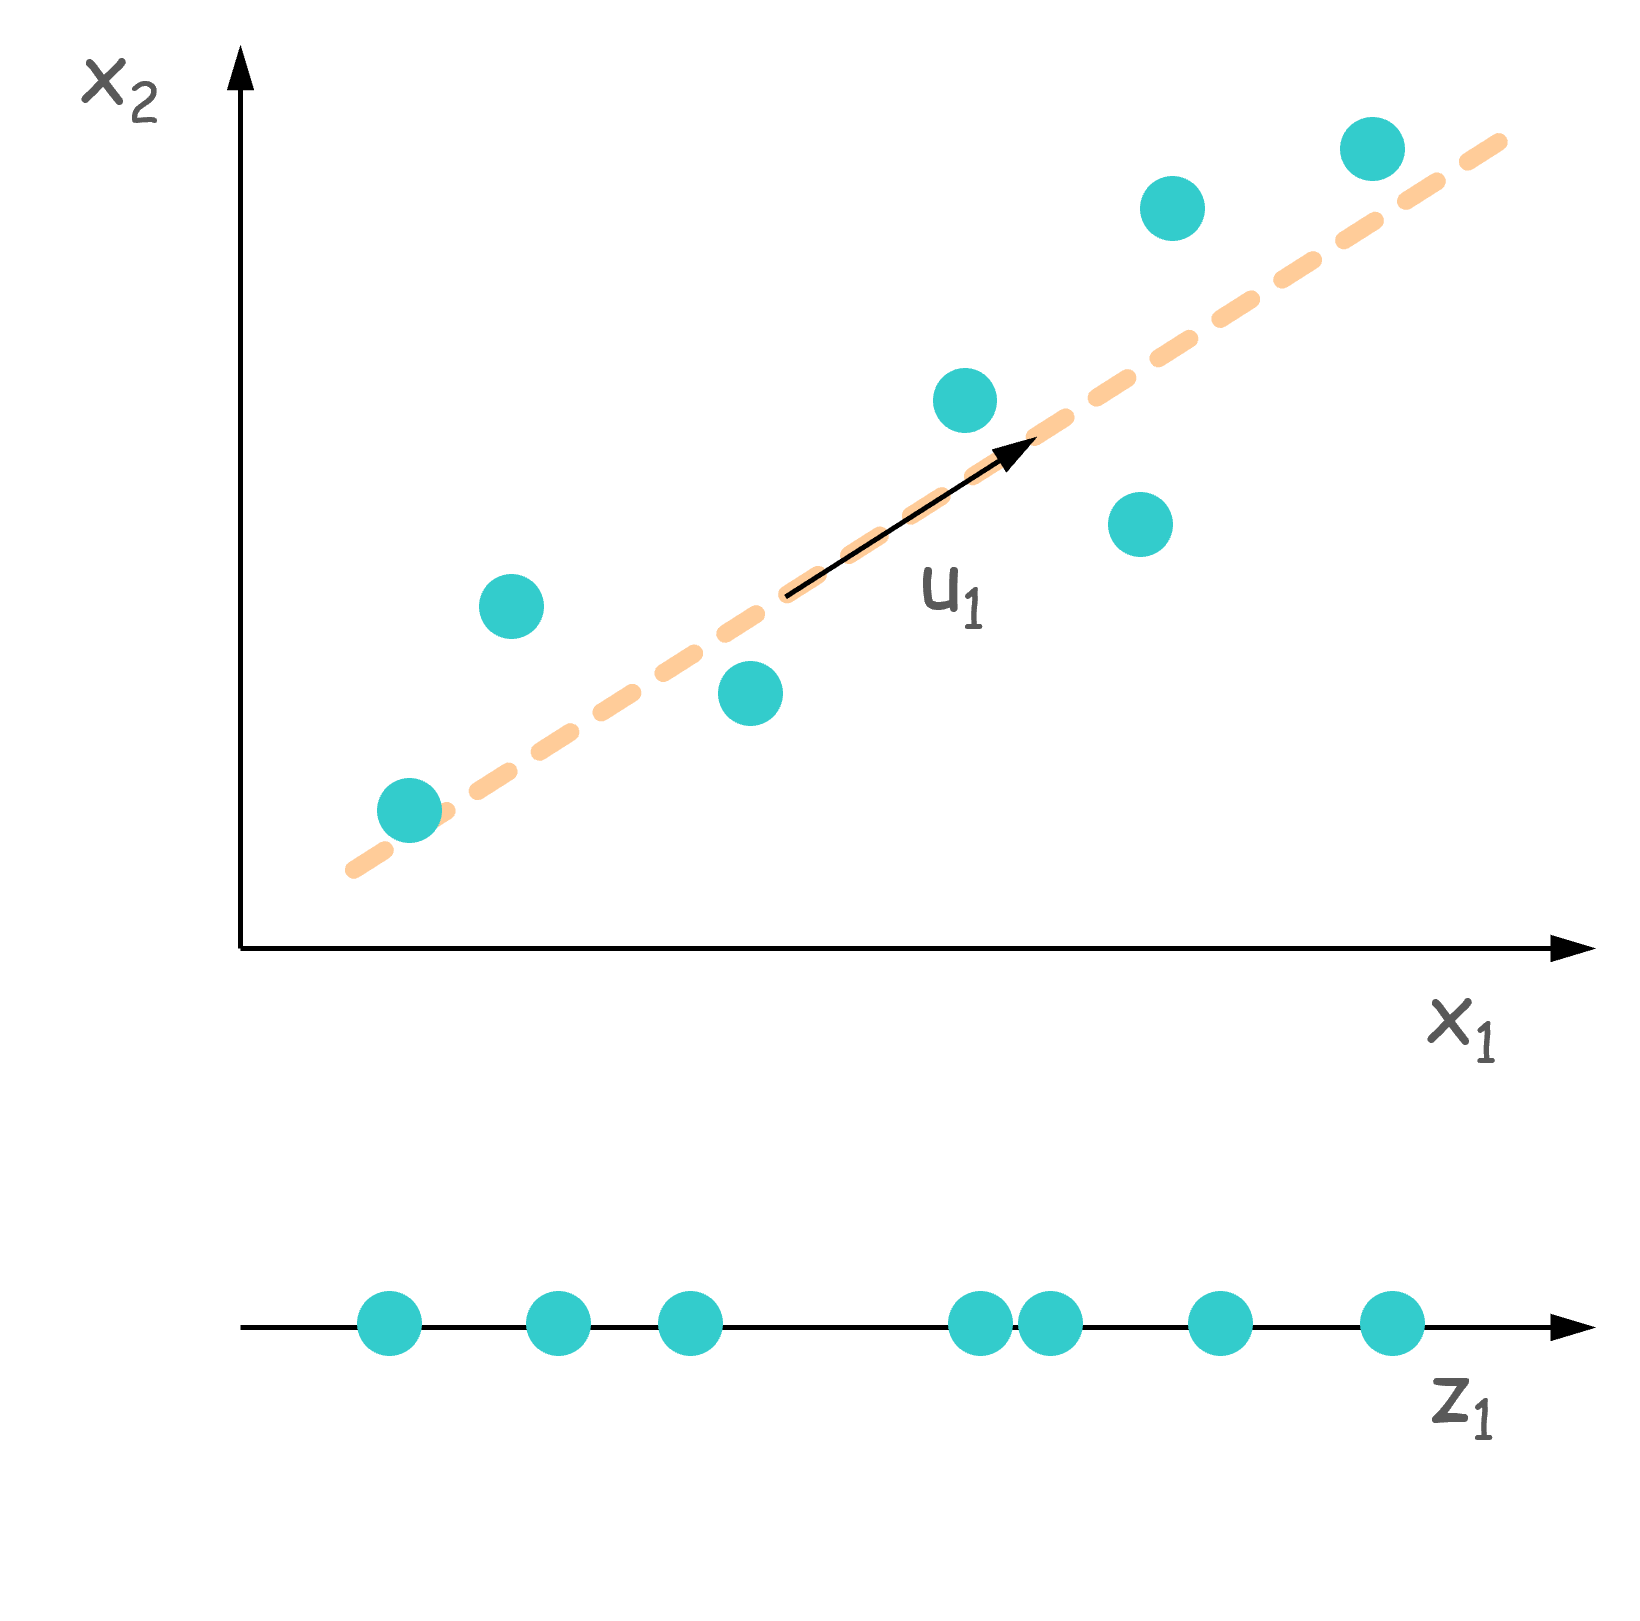
\includegraphics[width=2.2in]{./images/dimensionalityReduction2D.png}
            \caption{Reduction from 2D to 1D}
        \end{minipage}
        \begin{minipage}[t]{0.45\textwidth}
            \centering
            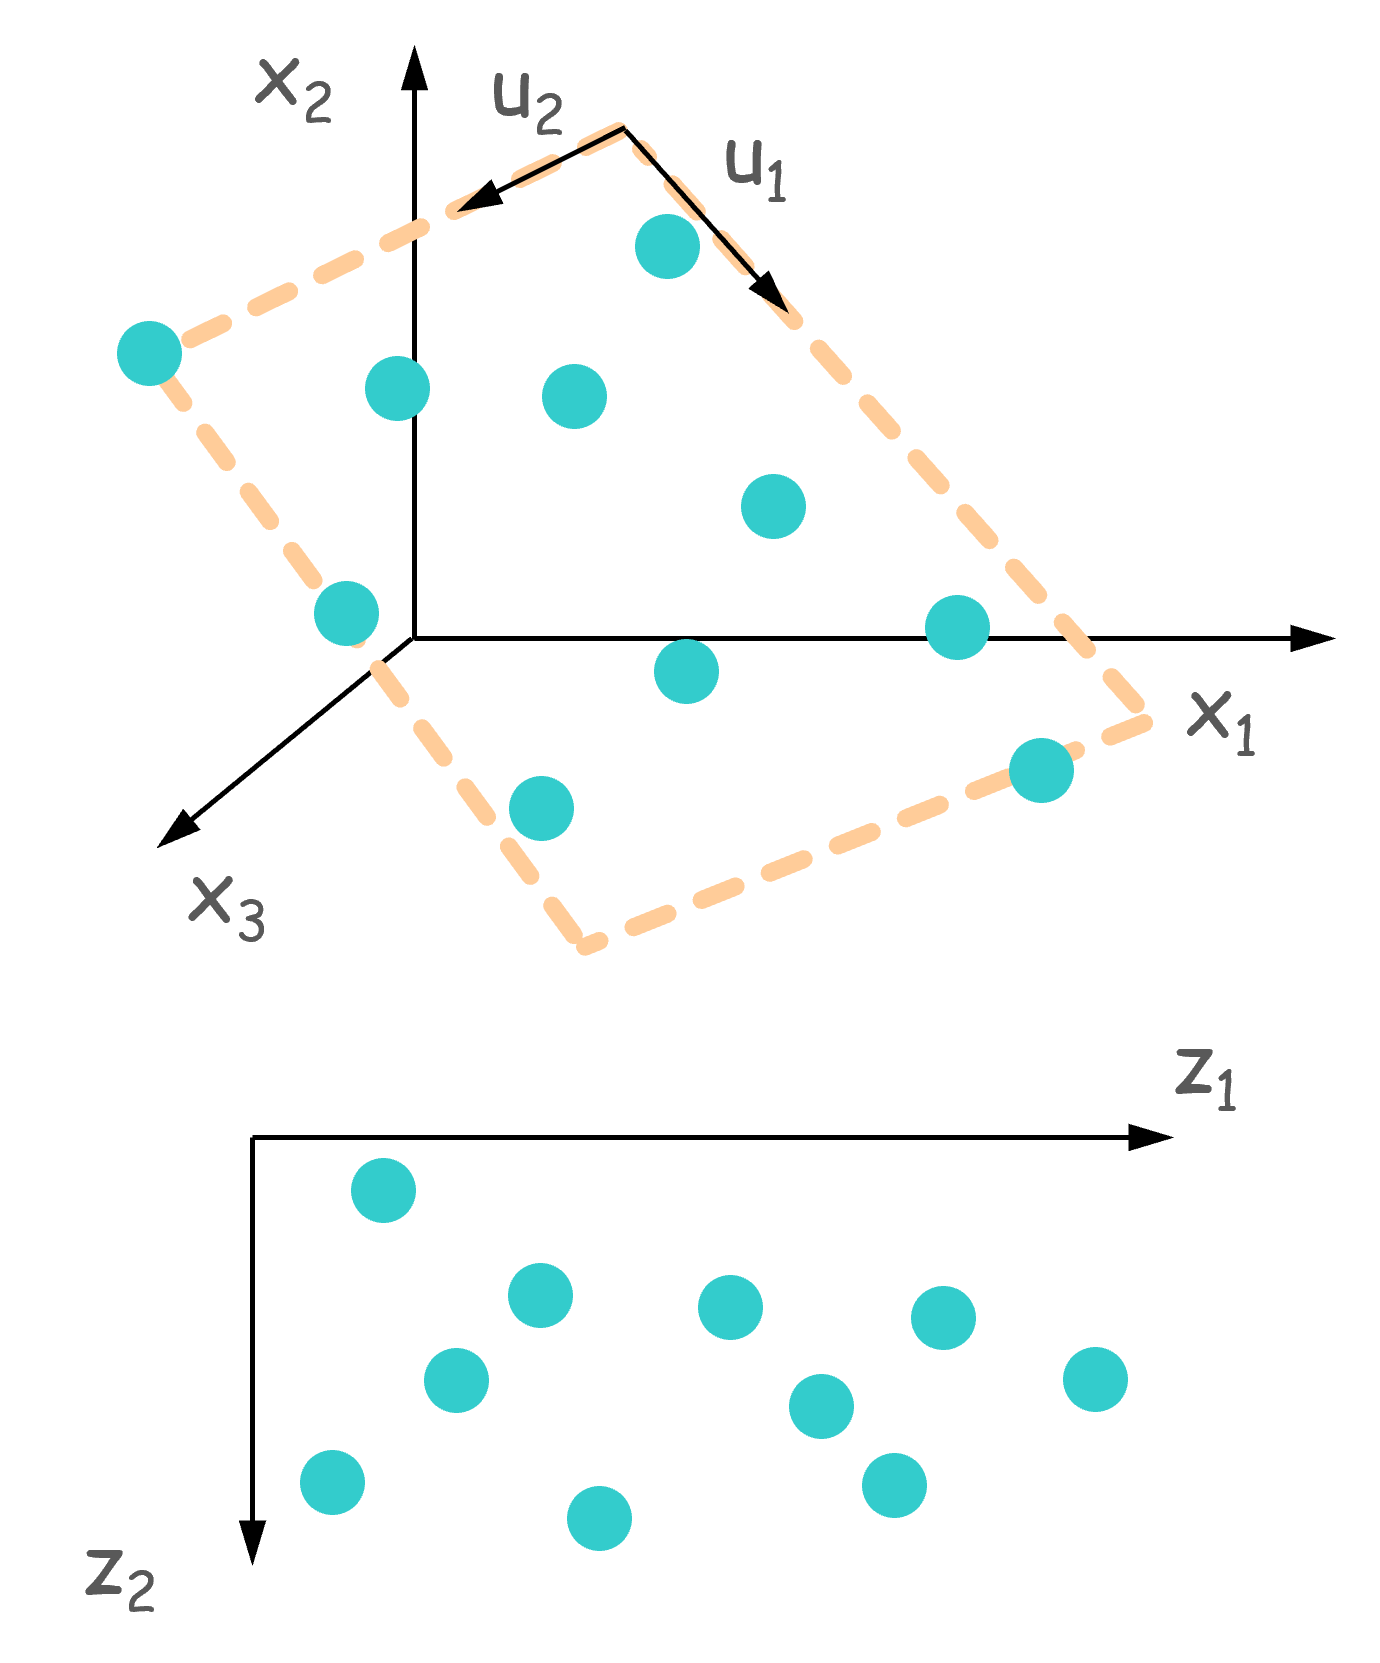
\includegraphics[width=2.2in]{./images/dimensionalityReduction3D.png}
            \caption{Reduction from 3D to 2D}
        \end{minipage}
    \end{figure}

    \item To reduce training data from n­‐dimension to k­‐dimension, find $k$ vectors
    \begin{equation}
        u^{(1)}, u^{(2)}, \dots, u^{(k)}
    \end{equation}
    onto which to project the data, so as to minimize the projection error.

    \item PCA is not regression
    \begin{figure}[!htbp]
        \centering
        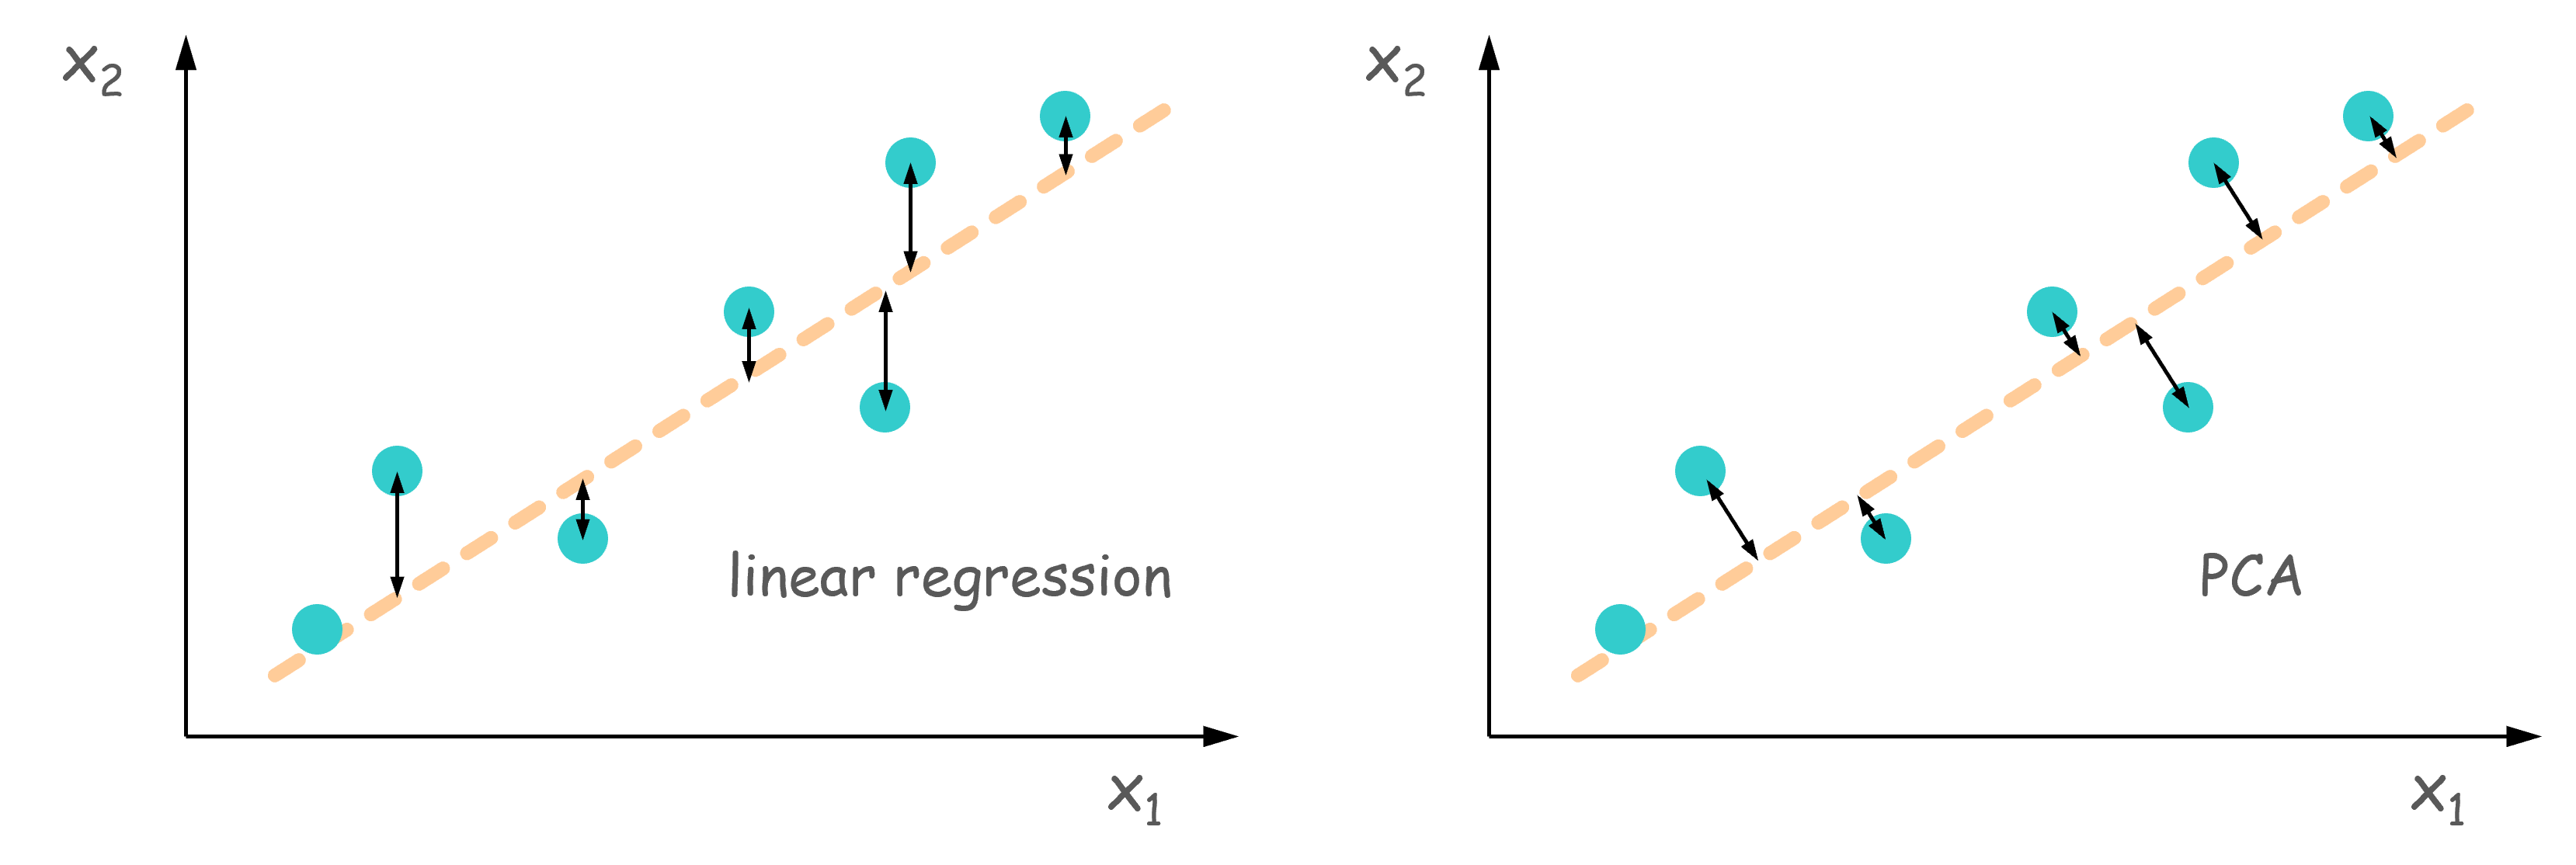
\includegraphics[width=4.4in]{./images/pcaVersusLinearRegression.png}
        \caption{PCA versus linear regression}
    \end{figure}
\end{itemize}


\section{Algorithm}
\begin{enumerate}
    \item Mean normaliza1on and feature scaling
    \begin{equation}
        x^{(i)} \coloneqq \frac{x^{(i)}-\mu^{(i)}}{s^{(i)}}
    \end{equation}
    where $\mu^{(i)}$ is the average of all the values for feature $i$ and $s^{(i)}$ is the range of values, or $s^{(i)}$ is the standard deviation.
    
    \item Compute \emph{covariance matrix}
    \begin{equation}
        \mathbf{C}_{n \times n} = \frac{1}{m}\sum_{i=1}^{m}{ {\mathbf{x}^{(i)}}^T \mathbf{x}^{(i)} } = \frac{1}{m}\mathbf{X}^T \mathbf{X}
    \end{equation}
    
    \item Compute \emph{eigenvectors} by \emph{singular value decomposition}
    \begin{equation}
        \mathbf{C}_{n \times n} = \mathbf{U}_{n \times n} \mathbf{\Sigma}_{n \times n} \mathbf{V}^T_{n \times n}
    \end{equation}
    Here $\mathbf{U}$ is a complex unitary matrix, the columns of which are orthogonal unit vectors called the left singular vectors of $\mathbf{C}$; 
    and $\mathbf{\Sigma}$ is an rectangular diagonal matrix of positive numbers $\sigma\left(k\right)$ called the singular values of $\mathbf{C}$; 
    and $\mathbf{V}$ is a complex unitary matrix whose columns are orthogonal unit vectors either called the right singular vectors of $\mathbf{C}$.

    \item Rearrange the eigenvectors and eigenvalues. 
    Sort the columns of the eigenvector matrix $\mathbf{U}$ and eigenvalue matrix $\mathbf{\Sigma}$ in order of decreasing eigenvalue.
    
    \item Select a subset of the eigenvectors as basis vectors
    \begin{equation}
        \mathbf{U}_{n \times n} = 
        \left[\begin{array}{ccccccc}
             |  &  |  &  |  &       &  |  &       &  |  \\ 
            u_1 & u_2 & u_3 & \dots & u_k & \dots & u_n \\
             |  &  |  &  |  &       &  |  &       &  |  \\ 
        \end{array}\right] = 
        \left[\begin{array}{ccc}
                         &       &  |  \\ 
            \mathbf{U}_k & \dots & u_n \\
                         &       &  |  \\ 
        \end{array}\right]
    \end{equation}
    
    Typically, choose $k$ to be smallest value so that
    \begin{equation}
        \frac{\sum_{i=1}^k \sigma_{ii}}{\sum_{i=1}^m \sigma_{ii}} \geq 0.9
    \end{equation}
    It means $90\%$ of variance retained.

    \item Project the data onto the new basis
    \begin{equation}
        \mathbf{Z}_{m \times k} = \mathbf{X}_{m \times n} \mathbf{U}_{k, n \times k}
    \end{equation}
    
    \item Recover an approximation of the original data that has been reduced to K dimensions
    \begin{equation}
        \mathbf{X}_{m \times n} = \mathbf{Z}_{m \times k} \mathbf{U}_{k, n \times k}^T
    \end{equation}
\end{enumerate}